%&glplain
\documentclass[12pt,a4paper]{article}
%\usepackage{apalike}
%\usepackage[rflt]{floatflt}
\usepackage{hyperref}
\usepackage{amsmath,amsfonts,amssymb}
\renewcommand{\familydefault}{\sfdefault}
\usepackage{helvet}
\usepackage{parskip}		%% blank lines between paragraphs, no indent
\usepackage[pdftex]{graphicx}	%% include graphics, preferrably pdf
\usepackage{listings}

%\usepackage[pdftex]{hyperref}	%% many PDF options can be set here
%\usepackage{nomencl}
%\usepackage{listings}
%\usepackage{amssymb}
%\usepackage{amsmath}
%\usepackage{wrapfig}



\newif\ifpdf
\ifx\pdfoutput\undefined
\pdffalse % we are not running PDFLaTeX
\else
\pdfoutput=1 % we are running PDFLaTeX
\pdftrue
\fi

\ifpdf
\usepackage[pdftex]{graphicx}
\else
\usepackage{graphicx}
\fi

\ifpdf
\DeclareGraphicsExtensions{.pdf, .jpg}
\else
\DeclareGraphicsExtensions{.eps, .jpg}
\fi


\setlength{\textwidth}{14.66cm} % height of main text
\setlength{\textheight}{22.2cm}    % width of text


\usepackage{nomencl}
\makenomenclature


\def\@@@nomenclature[#1]#2#3{% \def\@tempa{#2}\def\@tempb{#3}% \protected@write\@glossaryfile{}%
{\string\glossaryentry{#1\nom@verb\@tempa @{\nom@verb\@tempa}&% \begingroup\nom@verb\@tempb\protect\nomeqref{\theequation}%
            |nompageref}{\thepage}}%
     \endgroup
\@esphack}





\begin{document}

%: Title -----------------------------------------------
\thispagestyle{empty}
{\vspace*{-2.8cm} \hspace*{7.5cm} \includegraphics[width=75mm,viewport=0 0 235 85,clip]{Jacobs_LOGO_4C.pdf}}
\vspace{6.5cm}

% Author
{\noindent \large \textsf{Hang Yuan, Claudia Voelcker-Rehage, Lena H\"ubner, Herbert J\"ager, Benjamin Godde }} \\
\\

% Title
{\noindent \LARGE \bf \textsf{Resting State EEG Classification for Motor Learning Skills Using Echo State Networks}} \\
\vfill

% Report number
{\noindent \LARGE \textsf{Technical Report No. 36}} \\
% Month and year (e.g. May 2007)
{\noindent \textsf{August 2017}} \\
{\hspace*{-3.17cm} \rule[3mm]{\textwidth}{0.75pt}} \\
{\LARGE \textsf{School of Engineering and Science}} \\
% ----------------------------------------------------



\newpage
\thispagestyle{empty}

{ 
\noindent
\huge {\bf Main Title} \\
\\
\Large{sub title}\\
\normalsize

\vspace{1cm}

\noindent
{\bf Hang Yuan, Claudia Voelcker-Rehage, Lena H�bner, Herbert J�ger, and Benjamin Godde  }\\
\\
{\it 
School of Engineering and Science\\
Jacobs University Bremen gGmbH\\
Campus Ring 12\\
28759 Bremen\\
Germany\\ 
\\
E-Mail: \href{mailto: hang.yuan@epfl.ch}{ hang.yuan@epfl.ch}\\
\url{http://bgodde.user.jacobs-university.de/} 
} \\


}



\section*{Abstract}
EEG \nomenclature{\textbf{EEG}}{Electroencephalogram} records the electrical activities 
from the scalp surface via electrodes. As a modern medical imaging technique, 
it has been proven to be useful in many different fields. Clinical diagnosis, 
psychotherapy, brain-computer interfaces \nomenclature{\textbf{BCIs}}{Brain-Computer Interfaces} and the pharmaceutical industry all have 
benefited from the insights that one can glean from EEG measurements. \\

However, there exist various difficulties such as uniqueness of individuals, large volume of 
data and influences of artifacts that prevent us from extracting useful information from those 
measurements, and thus more involved analytical tools are needed. Recurrent Neural Networks
 \nomenclature{\textbf{RNNs}}{Recurrent Neural Networks}
are particularly suitable for dealing with EEG because these networks can capture the critical spatiotemporal characteristics
that EEG contains. \\

In this project, we successfully applied
 Echo State Networks \nomenclature{\textbf{ESNs}}{Echo State Networks} to classify 
 the  people's motor learning skills, \nomenclature{\textbf{MLS}}{ Motor Learning Skills} given the resting state EEG recording. We also discovered some evidence for the existence of different neurological groups with respect to people's motor learning skills. 

%: Table of Contents
\newpage
\thispagestyle{empty}
\tableofcontents


%: Sections
\newpage
\setcounter{page}{1}


\section{Introduction}


Given the long history of EEG studies, we have already decoded its relationships with a few brain processes like one's motor learning, motor imagery performance and even intelligence \cite{zhang2015efficient} \cite{ozdenizci2016resting}\cite{Doppelmayr2002289}.  Pursuing this line of inquiry this guided research plans to investigate if there exists a correlation between EEG signal and subjects' Motor Learning Skills (MLS), a latent variable that we will introduce more formally later.


Echo State Networks (ESNs) \cite{jaeger2001echo} are the more engineering favored reservoir computing method that was
independently discovered with Liquid State Machines \cite{maass2002real}, which concern more the computational
neuroscience's perspectives. We are mainly interested in the engineering problems, and thus solely touch on ESNs.
ESNs are a type of Recurrent Neural Network (RNN), which have a few notable advantages over traditional methods
for a sequence learning task (EEG classification)  \cite{lipton2015critical}. Static methods like Support Vector 
Machines (SVMs) and \nomenclature{\textbf{SVMs}}{Support Vector Machines} Feed-Forward Neural Networks (FNNs) 
  \nomenclature{\textbf{FNNs}}{Feedforward Neural Networks} have 
achieved excellent results on numerous learning tasks without explicitly modeling sequentiality. They can even
combine inputs within a windowed time frame for a model to encode the time dependency. Nevertheless, these static models cannot answer the questions about the events that occur outside the binned time steps. That is where RNNs come to rescue.
RNNs are a kind of neural networks whose units form directed cycles. The input is of the form $(x^1, x^2, \dots, x^T)$
and the corresponding labels for each time step is of the form $(y^1, y^2, \dots, y^T)$, where T is the number of time steps we have. 

It is empirically difficult to train RNNs mainly due to vanishing gradient and exploding gradient \cite{bengio1994learning}. Standard methods like backpropagation through time and real time recurrent learning suffer from the vanishing gradients since they both use the error gradient
taken from the objective function, and the gradient values become very small already after several steps. Among others, there are two approaches to avoid the exploding and vanishing gradients problem in RNN architectures: (i) In the Deep Learning\nomenclature{\textbf{DL}}{Deep Learning}  approach, exemplified by LSTMs \cite{Hochreiter1997lstm}, the problem is alleviated by utilizing additional structures of ``memory cell'' and gating mechanism, and (ii) in the Reservoir Computing approach, exemplified by ESNs, the problem is avoided by not learning the recurrent and input weights. In this report, we use the ESNs as our RNN architecture. We deter the discussion why ESNs are in favored for the EEG classification tasks to later sections.






ESNs give us an easy solution to the above issues while maintaining RNNs' power as we desire. ESNs are constructed using random weights for internal connections, which are fixed throughout the training process. It 
suffices to have a linear readout function for the output weights on the network responses which are simulated in the training.
Because of ESNs' simplicity, we can focus more on the understanding of the nonlinear dynamical systems which we train the models on.

So far, there have been several successful applications of RNNs or ESNs on EEG data analysis. Epileptic seizures disorder is a popular application of such techniques. We can build a warning system for the patients to be informed about an upcoming episode using EEG classification. Furthermore, the doctors can use the EEG model for epileptic activities to evaluate the treatment effectiveness \cite{buteneers2008real} \cite{naderi2010analysis}.  RNNs have also been used to detect Alzheimer's disease early on and other neurological degeneration  \cite{petrosian2001recurrent}\cite{ubeyli2008multiclass}. 

In this guided research, we have two objectives: one is of biological interest, finding out the association between resting state EEG and MLS,
and the other is of engineering interest: investigating the limitations and effectiveness of ESNs on EEG like data.

\section{Theoretical Frameworks}
\subsection{Echo State Networks (ESNs)}
We now introduce the general architecture of ESNs. In this section, we mainly  follow the notations from \cite{jaeger2001echo}\cite{lukovsevivcius2012practical} to keep things consistent. ESNs are mostly used for temporal supervised learning. We will present the setup in discrete time domain, denoting each time step as $ n = 1, 2, 3, \dots, T $, which leads the input signal to be $ \mathbf{u}(n) \in \mathbb{R}^K := (u_1(n), \dots, u_K(n))^\intercal$ and the teacher signal to be 
$ \mathbf{y^{target}}(n) \in \mathbb{R}^{N_y} := (y^{target}_1(n), \dots, y^{target}_{N_y}(n))^\intercal$. The model generates output $\mathbf{y} \in R^{N_y}$ to mimic the behavior of $\mathbf{y}^{target}$.

\begin{figure}[h]
	\centering
	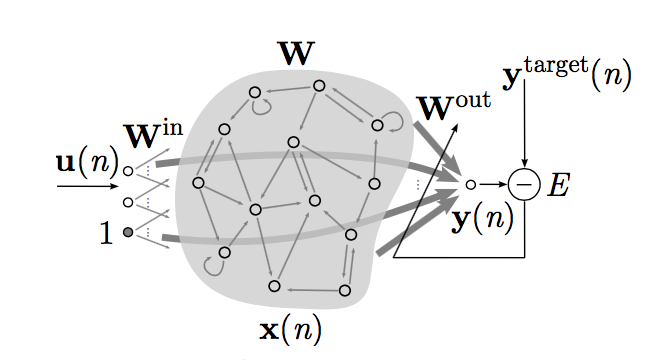
\includegraphics[width=0.8\textwidth]{img/esn_archi.png}
	%\caption{A basic ESNs architecture taken from \cite{jaeger2001echo}. The network consists
	%of three layers, an input layer of size K, an internal reservoir of size N and an output layer of size L.}
       \caption{A basic ESNs architecture taken from \cite{lukovsevivcius2012practical}.}
\end{figure}

As shown in Figure 1, the three different layers in the network have intermediate connections with each other, and sometimes they can even have feedback projections onto themselves. The black lines are the necessary connections, and the dotted ones are the optional connections. A typical minimal network graph will require three kinds of connections whose weights are expressed as: the input to the reservoir $\mathbf{W^{in}}$ , the internal connections among the units of the reservoir $\mathbf{W}$ and the reservoir to the output units $\mathbf{W^{out}}$. Optional input-to-output connections will increase the performance slightly at the cost of longer training time \cite{davidverstraeten2009}, and the optional output feedback loops to the internal units or to the output units themselves are used in signal simulation or to increase memory span\cite{maass2007computational}. In our experiment, since we do not need to simulate any time series, no back-projection is used.

\paragraph{Propagation steps} At each time step, the internal units are updated using leaky-integrated equations:
\begin{align}
\mathbf{\hat{x}} (n + 1) &= \mathbf{f}(\mathbf{W^{in}[1; u}(n+1)] + \mathbf{Wx}(n)) \\
\mathbf{x}(n + 1) &= (1 - \alpha)\mathbf{x}(n) + \alpha \mathbf{\hat{x}}
\end{align}
where $\mathbf{x(n + 1)} \in \mathbb{R}^{N_x}$ is reservoir neuron activations, $N_x$ is the number of reservoir units, $\mathbf{\hat{x}(n + 1)} \in \mathbb{R}^{N_x}$ is the reservoir update,  $\alpha$ is the leaky coefficient, $[-;-]$ represents vector(matrix) wise concatenation, $\mathbf{f}$ is the activation function for the internal units and 1 is the bias term. Threshold functions, hyperbolic tangent function or sigmoid function are all candidates for the activation function. We use hyperbolic tangent in the implementation.  As for the output, the update rule is:
\begin{align}
\mathbf{y} (n + 1) = \mathbf{W^{out}}[1; \mathbf{u}(n+1);\mathbf{x}(n+1)]
\end{align}


\paragraph{Training steps} We start with some state $\mathbf{x}(0)$ and then use equation (1) and (2) to simulate the output signal until $T_{max}$. We then discard the simulation results until $n_{min}$ when, the network dynamics become stable. From this point on, we assume time 0 is the first time step after $n_{min}$. The Error function $E$ usually measures the Root Mean Square Error (RMSE) \nomenclature{\textbf{RMSE}}{Root Mean Square Error} defined as:
\begin{align}
E(\mathbf{y, y^{target}}) = \frac{1}{N_y} \sum^{N_y}_{i=1} \sqrt{\frac{1}{T} \sum^{T}_{n=1}(y_i(n) - y_i^{target}(n) )^2}
\end{align} 
It suffices to run a linear regression on the output signal to minimize the MSE between the predictions and the teacher signals. Nevertheless, after we concatenate the simulation outputs into a matrix $\mathbf{X}$, $\mathbf{X}$ is most likely overdetermined because quite often $ T > N_x $. $N_x$ is the number of the reservoir units. It follows that we need to make use of a few techniques to solve the system. We now look at two of such methods, ridge regression and pseudoinverse inverse.

Ridge regression yields:
\begin{align}
\mathbf{W^{out}} = \mathbf{y^{target}X^\intercal (XX^\intercal } + \beta \mathbf{I})^{-1}
\end{align}
where $\mathbf{I}$ is an identity matrix and $\beta$ is a regularization coefficient. 

\paragraph{Prediction steps} Implant the trained $\mathbf{W^{out}}$ in the readout layer and do the propagation steps for any new input data. 
 
 \paragraph{Networks parameters} There are three model parameters that define ESNs, namely $(\mathbf{W^{in}, W}, \alpha )$. There are other important parameters for the network: the size of internal units, sparsity, spectral radius of $\mathbf{W}$ and scaling of $\mathbf{W^{in}}$ \cite{lukovsevivcius2012practical}. To achieve satisfying performance, one should consider the above factors in the design phase. We briefly list a few optimization techniques with respect to those parameters:
 \begin{itemize}
 	\item Spectral radius $\rho$: The critical parameter that ensures the effectiveness of ESNs is spectral radius. This is because, for ESN approach to work, the reservoir must satisfy the ``echo state property'' : given a long enough input sequence, the current state is uniquely defined by the previous history such that sequence and the network state $\mathbf{x}(n)$ should not rely on the information that occurs before the initial state \cite{jaeger2001echo}. In most cases, $\rho(\mathbf{W}) < 1$ guarantees the echo state property. Implementation wise, we can first compute the spectral radius of $\mathbf{W}$, and then divide the matrix itself with this value to obtain the unit spectral radius which can be easy to use in the tuning phase.

%There are a few assumptions that ESNs approach has, one of which is the echo state property. 	
%This property states that the network can be viewed as a function of left-infinite history $\mathbf{u}(n), \mathbf{u}(n-1), \dots $, so to say we have an echo function $EC$,
% 	\begin{align}
 %	EC = (e_1, \dots, e_N) \text{ where } e_i : U^{-\mathbb{N}} \implies \mathbb{R} 
 %	\end{align}
 %	in which $\dots, \mathbf{u}(n-1), \mathbf{u}(n) \in U^{-\mathbb{N}}$. For any left-infinite input sequence, the current state is determined by:
 %	\begin{align}
%	\mathbf{x}(n) = EC(\dots, \mathbf{u}(n - 1), \mathbf{u}(n))
 %	\end{align}
 
  	
  %Size of the reservoir $N_x$: In \cite{jaeger2001short}, the memory capacity (MC)  \nomenclature{\textbf{MC}}{Memory Capacity} of an $N$-unit RNN with linear output to recall an i.i.d. input has been shown to be bounded by $N$. It makes sense to have $N_x \geq N$ for the minimal setup. On the other hand, only when $T < 1 + N_u + N_x$, will we have a reservoir layer that's too large for the dataset. In general, the bigger the reservoir one uses, the better the performance will be. 
	
\item In general, the better the obtainable performance (provided appropriate regularization measures are taken against overfitting) \cite{lukovsevivcius2012practical}. On the other hand, only when $T < 1 + N_u + N_x$, will we have a reservoir layer that's too large for the dataset.
	
 	 	
 	 \item Leaking rate: The significance of this parameter stems from the discretization of continuous time update, which is described in equation (1) and (2). In the context of discrete time, we have:
 	 \begin{align}
 	 \frac{\Delta\mathbf{x}}{\Delta t} = \frac{\mathbf{x}(n+1) - \mathbf{x}(n)}{\Delta t} \approx \dot{\mathbf{x}} 
 	 \end{align}
 	 It becomes clear that the leaky rate $\alpha$ is the transformation piece between the discrete and continuous worlds. Changing $\alpha$ to match up with the change rate of $\mathbf{u}(n) \text{ and or } \mathbf{y}^{target}(n)$ is similar to resampling of inputs in order to achieve better performance \cite{schrauwen2007introduction}. 
 	 
 \end{itemize}


\subsection{Resting State Electroencephalogram (EEG)}
EEG measures the electrical activities from the scalp surface which are recorded via electrodes and other conductive media \cite{niedermeyer2005electroencephalography}. EEG is mostly influenced by the activity of the cerebral cortex that is close to the scalp surface. The EEG data records the relative voltage difference between electrodes and a reference electrode, that is usually placed in the middle of the scalp. There are two reasons why the raw voltage values are not of interest. First, the voltage values will change due to different choices of baseline subtraction. Secondly, the raw values will be hard to analyze because of the individuals' differences that may not play a role in the desired cognitive processes studies. \cite{cohen2014analyzing}

EEG has three temporal properties: resolution, precision and accuracy. Resolution reflects how many  data points are recorded per unit time, precision reflects how certain the measurements are and accuracy reflects the mapping between the timing of the EEG signals and the timing of the actual occurrences of the events \cite{cohen2014analyzing}. The temporal resolution is determined by the rate of acquisition. It enables one to extract frequency-band-specific features. Furthermore, brain waves are separated into five groups based on their frequency domains. Their corresponding frequency domains are usually associated with:
\begin{itemize}
	\item $  \gamma $ waves: $freq \in (30, 80) Hz$
	\item $ \beta $ waves: $freq \in (13, 30) Hz$
	\item $ \alpha $ waves: $freq \in (8, 13) Hz$
	\item $ \theta $ waves: $freq \in (4, 8) Hz$
	\item $ \delta $ waves: $freq \in (0.5, 4) Hz$
\end{itemize}
Figure 2 shows some examples of how brain waves of different frequency bands look like.
\begin{figure}[h]
	\centering
	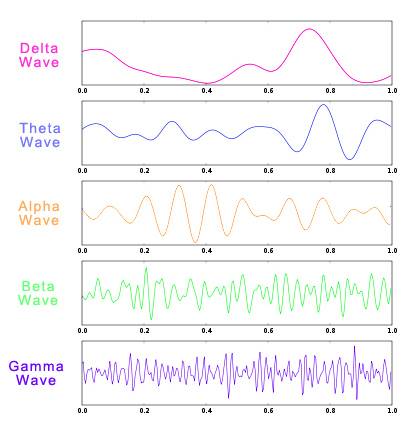
\includegraphics[width=0.5\textwidth]{img/waves.png}
	\caption[Caption for LOF]{Brain waves visualization based on different frequency bands.\footnotemark}
%	\caption{}
\end{figure}
\footnotetext{Figure taken from the site: http://www.brainworksneurotherapy.com/what-are-brainwaves}
EEG is a good technique to study the brain for a few reasons: This method records the brain dynamics at the time when the cognitive events happen; Secondly, EEG directly measures the brain activity. Changes in voltage potentials are due to neurological behavior at the neuron population level; Lastly, EEG contains rich information and is multidimensional. It not only has the spatiotemporal information, but also frequency, power and phase as features that give us ample knowledge about the internal brain activities. \cite{cohen2011s}

\paragraph{Properties of EEG features for analytics} 
These are paramount factors to consider when one analyzes EEG signals.
\begin{itemize}
	\item Noise and signal: EEG signals are noisy, and the noises are often hard to discriminate. One will have to find the fine line between removing too much useful information and having noisy data depending on the given task. Figure 3 is a good demonstration of the signal and noise relationship.
	\begin{figure}[h]
		\centering
		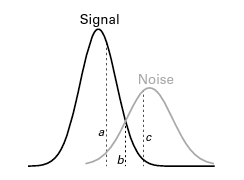
\includegraphics[width=0.5\textwidth]{img/noise.png}
		\caption{This plot shows the interconnected relationship between signal and noise in EEG (taken from \cite{cohen2014analyzing}). The x-axis is the degree of data cleaning that we conduct and the y-axis is the leftover for signal and noise after the cleaning. We can see the distribution of signal and noise with respect to the level of preprocessing. Area left to a implies there is little noise left, area between a and b has a mixture of both noise and signal and the area right to c has mostly noise.}
	\end{figure}
	\item Non-stationarity: EEG signals can change quickly over time.
	\item Small training sets: Due to the costs of collecting data from subjects, the training sets are oftentimes 
	smaller than ideal.
\end{itemize}

\paragraph{Preprocessing}
\begin{itemize}
	\item Filtering: One wants to have high-frequency artifacts and low-frequency drifts removed in this step.
	It is recommended to use high-pass filter at 0.1Hz or 0.5Hz to get rid of the slow drifts \cite{cohen2014analyzing}.
	\item Spatial filtering: Spatial filtering is needed when you want to localize a result and to eliminate topological features of the data. For instance, if an experiment requires the subjects to conduct some tasks that involve multiple brain regions, it would be otherwise difficult to isolate the active regions without spatial filtering. \cite{cohen2014analyzing}
\end{itemize}

It is worth noting that there is a trend in Machine Learning (ML)  \nomenclature{\textbf{ML}}{Machine Learning} that tries to construct end-to-end models without any preprocessing of the data nowadays. People often use a class of techniques called Deep Learning (DL). DL methods compose multiple levels of representational simple and nonlinear layer. Each layer learns at different degrees of abstraction. With enough layers, the models can learn how to discriminate important aspects of data from other variations. DL has made lots of advances in solving challenging problems. In the recent decade, DL has produced competition winning approaches in imaging recognition \cite{krizhevsky2012imagenet}\cite{farabet2013learning} and promising methods for sequence learning tasks in natural language processing \cite{bordes2014question} \cite{luong2014addressing}. However, DL methods are not suitable for EEG data processing, because DL methods usually have many free parameters, and it is simply hard to collect enough EEG data for the training purpose. In robotics, although it is also difficult to obtain real world data, people can simulate the training data in a physics engine because the mechanics of robots' interactions and the real world are well understood. Unfortunately, this is not possible for EEG data yet, since we simply do not understand the brain well enough to have a simulator for the brain's underlying mechanisms.



\paragraph{Artifacts}
Artifacts originate from numerous sources in an EEG study, such as blinks, muscle movements and wire noise. Note that EEG is not an error-free measurement technique and we do not know all sources of error. Fortunately, after some reasonable preprocessing, most analytics tools are robust enough to the leftover noise. Independent Components Analysis (ICA) is the common choice for artifacts removal. It essentially separates the source into different independent sources. Originally, ICA was meant to solve the blind source separation problem, trying to retrieve the independent sources $ \mathbf{s} = ({s_1(t), \dots, s_N(t)})$ \cite{comon1994independent}. The sources $\mathbf{s}$ is being mixed by an unknown matrix $\mathbf{A}$, such that the recorded $N$ mixture $ \mathbf{x} = ({x_1(t), \dots, s_N(t)})$ has the property that 
\begin{align}
\mathbf{x = As}
\end{align} 
ICA in the context of EEG records, separates the data at different electrodes into a sum of various temporally independent components \cite{jung2000removing}, and thus muscle movement, eye blinks and oculomotor activities can generally be detected and rejected.  Traditionally, artifacts detection from ICA need human experts to manually remove the corrupted components but this takes lots of time and training. Most of the ICA-based removal techniques require additional recording for a subject's artifact activity. For example using two eye electrodes to record eye movements and then do a correlation analysis to remove artifactual  components later on. In this project, we are using a fully automated method  Multiple Artifact Rejection Algorithm (MARA) \cite{Winkler2011}. MARA is a supervised-learning linear approach that learns from over 1k samples labeled by experts. Without using additional recordings, we are still able to automate the artifacts removal process. \nomenclature{\textbf{MARA}}{Multiple Artifact Rejection Algorithm} 


\paragraph{Classification overview}
There are five common types of classification algorithms in EEG analytics: linear classifiers, neural networks, nonlinear Bayesian, nearest neighbor and classifier combinations \cite{lotte2007review}. Here we will discuss two of them and their corresponding characteristics in EEG classification.

\begin{itemize}
	\item Linear classifiers: Linear Discriminant Analysis (LDA) \nomenclature{\textbf{LDA}}{Linear Discriminant Analysis} and SVMs are the most common linear classifiers in EEG analysis. LDA uses several hyperplanes to separate the data. It is cheap to compute and therefore a good candidate for online learning. SVMs also make use of hyperplane separation but they have a different objective, maximizing the margins between different class planes. SVMs have a few good properties, thanks to the regularization terms:  robustness for overfitting and tolerance to the curse-of-dimensionality \cite{bennett2000support}.
	
	\item Neural networks: Multilayer Perceptron (MLP) \nomenclature{\textbf{MLP}}{ Multilayer Perceptron} has been widely used in EEG classification \cite{anderson1996classification}\cite{palaniappan2005brain} due to its flexibility to adapt to different problems. However with noisy and non-stationary data like EEG, it is particularly prone to overfitting \cite{balakrishnan2005multilayer}, and thus it needs careful tuning and architecture design. We should pay special attention to the Gaussian classifier which is specifically created to process EEG data in Brain-Computer Interfaces (BCIs) \cite{millan2004noninvasive} \cite{millan2000local}. In this local neural classifier, each unit in the network is a Gaussian discriminator for each class prototype and if a class has several prototypes, only the nearest one is used. During training, units are pushed towards the EEG samples of the same class and are pushed away from the ones that do not belong to the same class. It has been shown that this kind of architecture is superior to MLP in terms of the rejection efficiency for uncertain samples \cite{millan2000local}. As for ESNs,  they have been used to construct a fast and reliable method for epileptic seizure detection \cite{buteneers2008real}, however, it is not clear how effective ESNs are in EEG classification when compared with other methods due to the lack of relevant study, nevertheless ESNs should still be a good choice for such a sequence learning task and we would like to explore its limitations in this regard.

\end{itemize}


\section{Motivation}
The main objective of this guided research lies in two folds, one is engineering oriented, and the other is physiology oriented:
\begin{itemize}
	\item Construct reliable and efficient ESNs to classify the EEG signals.
	\item Explore if there exists a relationship between resting state EEG and MLS. If such a relationship does exist, what can we say about that?
\end{itemize} 

So far the applications of ESNs being used as an EEG classifier are not extensive, although there have been a few in the past years on sequence learning tasks, classifications of real time moving objects \cite{mitul2013classification} and time series classification for the prediction of dialysis \cite{ongenae2013time}. On this note, we wish to summarize the proposed questions from the engineering perspective:
\begin{itemize}
	\item How tolerant ESNs are when dealing with noisy and non-stationary data like EEG, and when it is good enough to stop cleaning without compromising  useful information.  
	\item How ESNs can best handle time-variant features, more specifically how they deal with the drifting of amplitudes which can be slow and fast at different times?
	\item What kinds of tuning need to be done in order to avoid this situation, as training a classifier for EEG using neural networks is prone to over-fitting?
	\item Is it possible to adapt the reservoir distribution somehow such that the model is better suited for EEG classification?
\end{itemize}

Now we come to the physiological side. So far, stable resting brain activities have been shown to have correlations with personal traits like personality, intelligence and neurological disorder \cite{thatcher2005eeg}\cite{davidson2003affective}. We also know that there is a correlation between event-based computation and the preceding resting state EEG of that event, for instance, the strategy one uses in problem solving \cite{kounios2008origins}. There are more correlations to discover, and correlation between EEG and MLS is one of them. Merely by using a partial least squares regression model, one can already predict the motor skill acquisition well \cite{wu2014resting}. It would not surprise us if we can achieve better prediction performance using ESNs. Our hypothesis is that the MLS is related to resting state EEG in both young and old age groups. Along with this line of inquiry, this guided research is determined to tackle the following questions: 

\begin{itemize}
	\item Given the traits of each individual, what is a plausible definition for the MLS that both makes sense physiologically but will also work well for ESNs?
	\item What insights can we learn from the response activity in each internal unit of ESNs? Do the responses contain any critical information about the subjects like the biological age or the cognitive ability?
	\item Does compensation effect exist in old high-performing group?
\end{itemize}

\section{Experiments}
\begin{figure}[h]
	\centering
	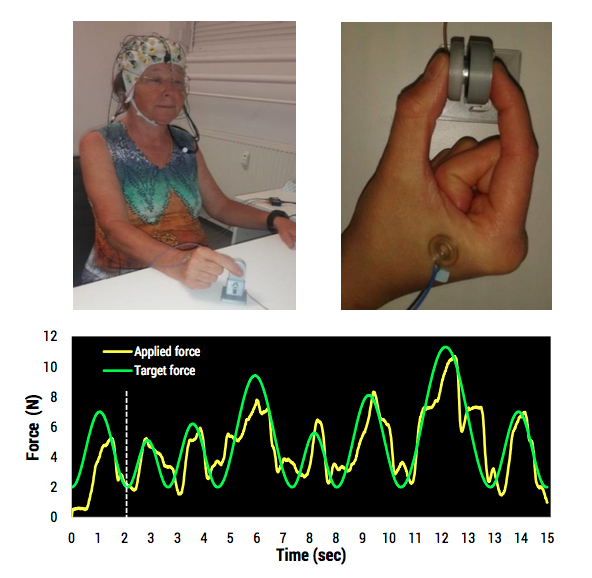
\includegraphics[width=0.8\textwidth]{img/subject.png}
	\caption{The top two images show how the force modulation task is performed, and the bottom image shows what a subject sees during the experiment (taken from \cite{subject2016}).}
\end{figure}

\paragraph{Data source} The EEG data was recorded by Professor Benjamin Godde and his research group for a motor learning study in older adults. 87 women participated in the study of which 55 were between the age of 67 and 83, and 32 were between the age of 19 and 29. The older participants were recruited using the contact information stored in a previous study at Jacobs University Bremen, and the younger participants were recruited using flyers and mailing lists. The subjects were asked to conduct a fine motor force modulation task, in which the subjects needed to apply some precise grip with dominant hand on a force transducer. The experiment setup is shown in the top two images of Figure 4. The performance of the force being applied can be seen on a monitor, on which both the target force and the actual force are shown to give feedbacks (Figure 4 bottom). The subjects needed to track the target force as close as he could. Irregular since wave pattern of eight waves were collected per trial, and eight trials made up a block. The target variable we have the pre-and-post training Root Mean Square Error (RMSE)  \nomenclature{\textbf{RMSE}}{Root Mean Square Error} from since wave two to wave seven.


\begin{figure}[h]
	\centering
	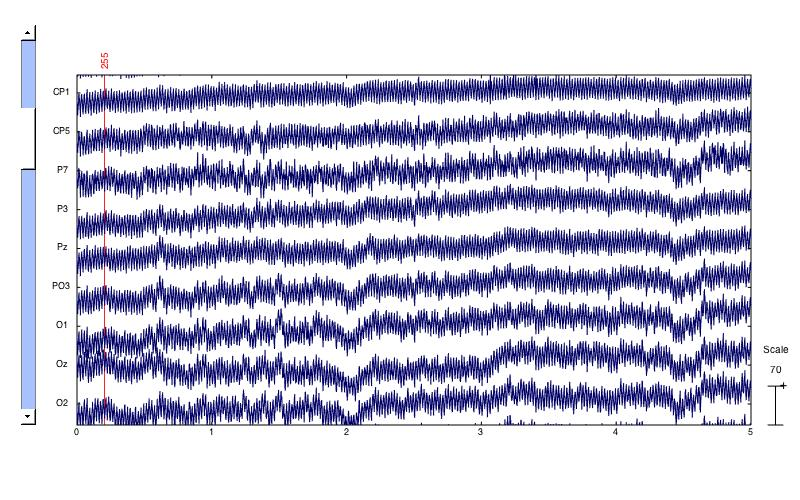
\includegraphics[width=1.0\textwidth]{img/visu.jpg}
	\caption{A clip of raw data for 8 channels across five seconds}
\end{figure}

  The resting-state EEG was recorded with 32 channels at a sampling rate of 2048 Hz. In Figure 5, one can see a short clip of the EEG recording for eight channels. Clearly, most of the signals demonstrate some periodic behaviors and on the lower half of the plot, channels like O1, Oz and O2 have more fluctuations within this time frame.  The recording machinery is an active electrode system (ActiveTwo, BioSemi, Amsterdam, Netherlands) mounted in an elastic nylon cap \cite{jasper1958ten}. The eventual usable data contains 79 subjects' resting EEG recordings for 80 seconds. There are 30 young subjects and 49 old subjects. The total EEG data is about 1.5 GB. In addition, for each subject, we have a few meta variables, some of which are going to compose MLA later on:
\begin{itemize}
	\item Biological traits: age and gender
	\item Age group: a binary class variable to denote if a participant belongs to the young or old group
	\item Moca: an indicator value for the risk of dementia
	\item $VO_2$ peak: peak oxygen consumption in a stationary bicycle task for fitness level measurement
	 \item MVC: max voluntary contraction, the max force between the thumb and index finger for 5 seconds 
	 \item PreRMSE and PostRMSE: the motor performance before and after the motor learning training
\end{itemize}

Since we are building a binary EEG classifier, the model construction pipeline is quite obvious. For this project, we follow the construction diagram in Figure 6. The whole experiment section mainly consists of three stages: preprocessing, model building and post-processing.

	\begin{figure}[!h]
	\centering
	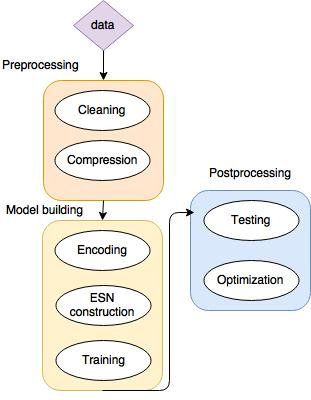
\includegraphics[width=0.40\textwidth]{img/dataflow.jpg}
	\caption{Data processing pipeline}
\end{figure}

	\paragraph{Preprocessing} As we already discussed in section 2, two of the main problems that an EEG classifier faces are the curse of dimensionality and low data-noise ratio. Therefore, cleaning and compression stages are necessary. For cleaning, we use a bandpass filter 0.5 - 79 Hz, then we apply ICA, in preparation for artifacts removal.\footnote{We run the runica version ICA in EEGLAB.}. After obtaining the independent components, we remove all the components that are marked as artifacts by MARA. Let us look at one example of MARA operates when being applied. 

	\begin{figure}[!h]
	\begin{center}
		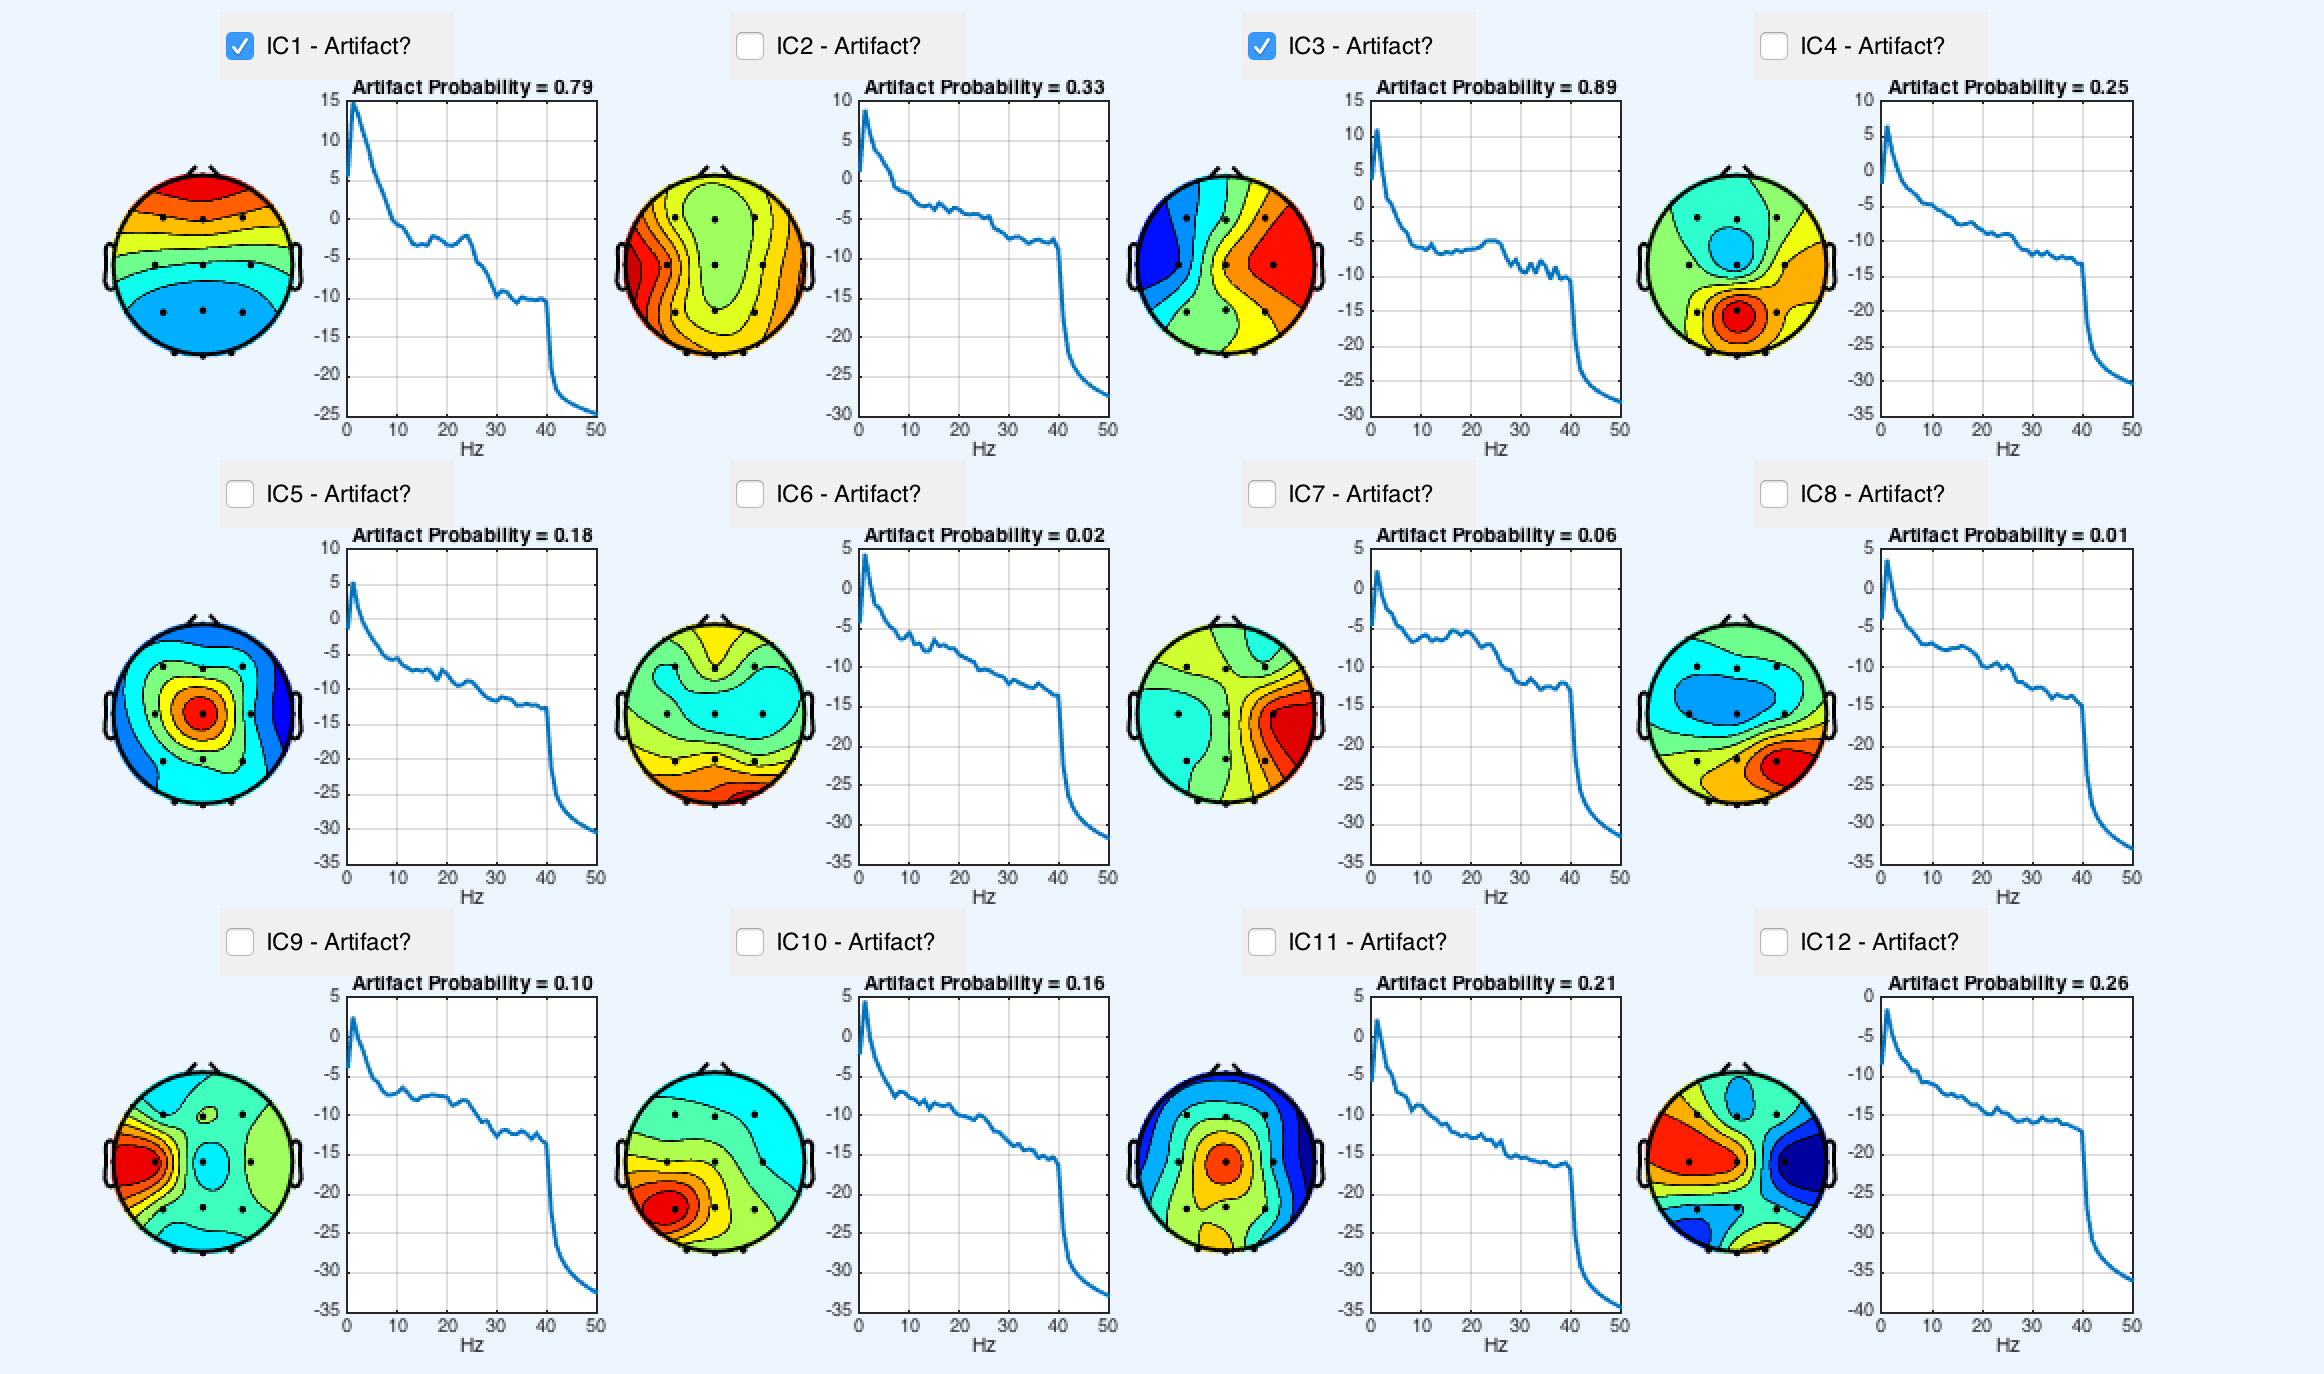
\includegraphics[width=\textwidth]{img/ica.png}
	\end{center}
	\caption{Artifact markers for a sample data stream by MARA are shown. MARA operates on the independent components. For each component, we have three things: a scalp map projection of this particular component (more red means more activity and more blue means lower activity), a power spectrum with artifact probability (the x axis is frequency in Hz, and the y axis is the magnitude in dB) and the if artifact label. }
\end{figure}
	In Figure 7, we have 12 independent components of a subject's recording. Component one and component three are marked as artifact with high probability. In the current setup, all components marked as artifacts are removed by default, but if one wants to be more careful, a threshold on probability can be used. In component one, there is a strong impulse in the frontal area which should be mainly due to eye movements, and in component three on the right hemisphere where no brain tissue exists, we also have lots of activities, and thus it is not surprising that these two components are marked as artifacts. In all the power spectrum plots, we see a sharp decrease around 40-50 Hz due to an omission of notch filter in the preprocessing that is to be done. After the artifacts are removed and proper filtering, the power spectrum should demonstrate spectral peaks at typical EEG frequencies, and the scalp maps should be dipole-like.  


		\begin{figure}[!h]
			\begin{center}
				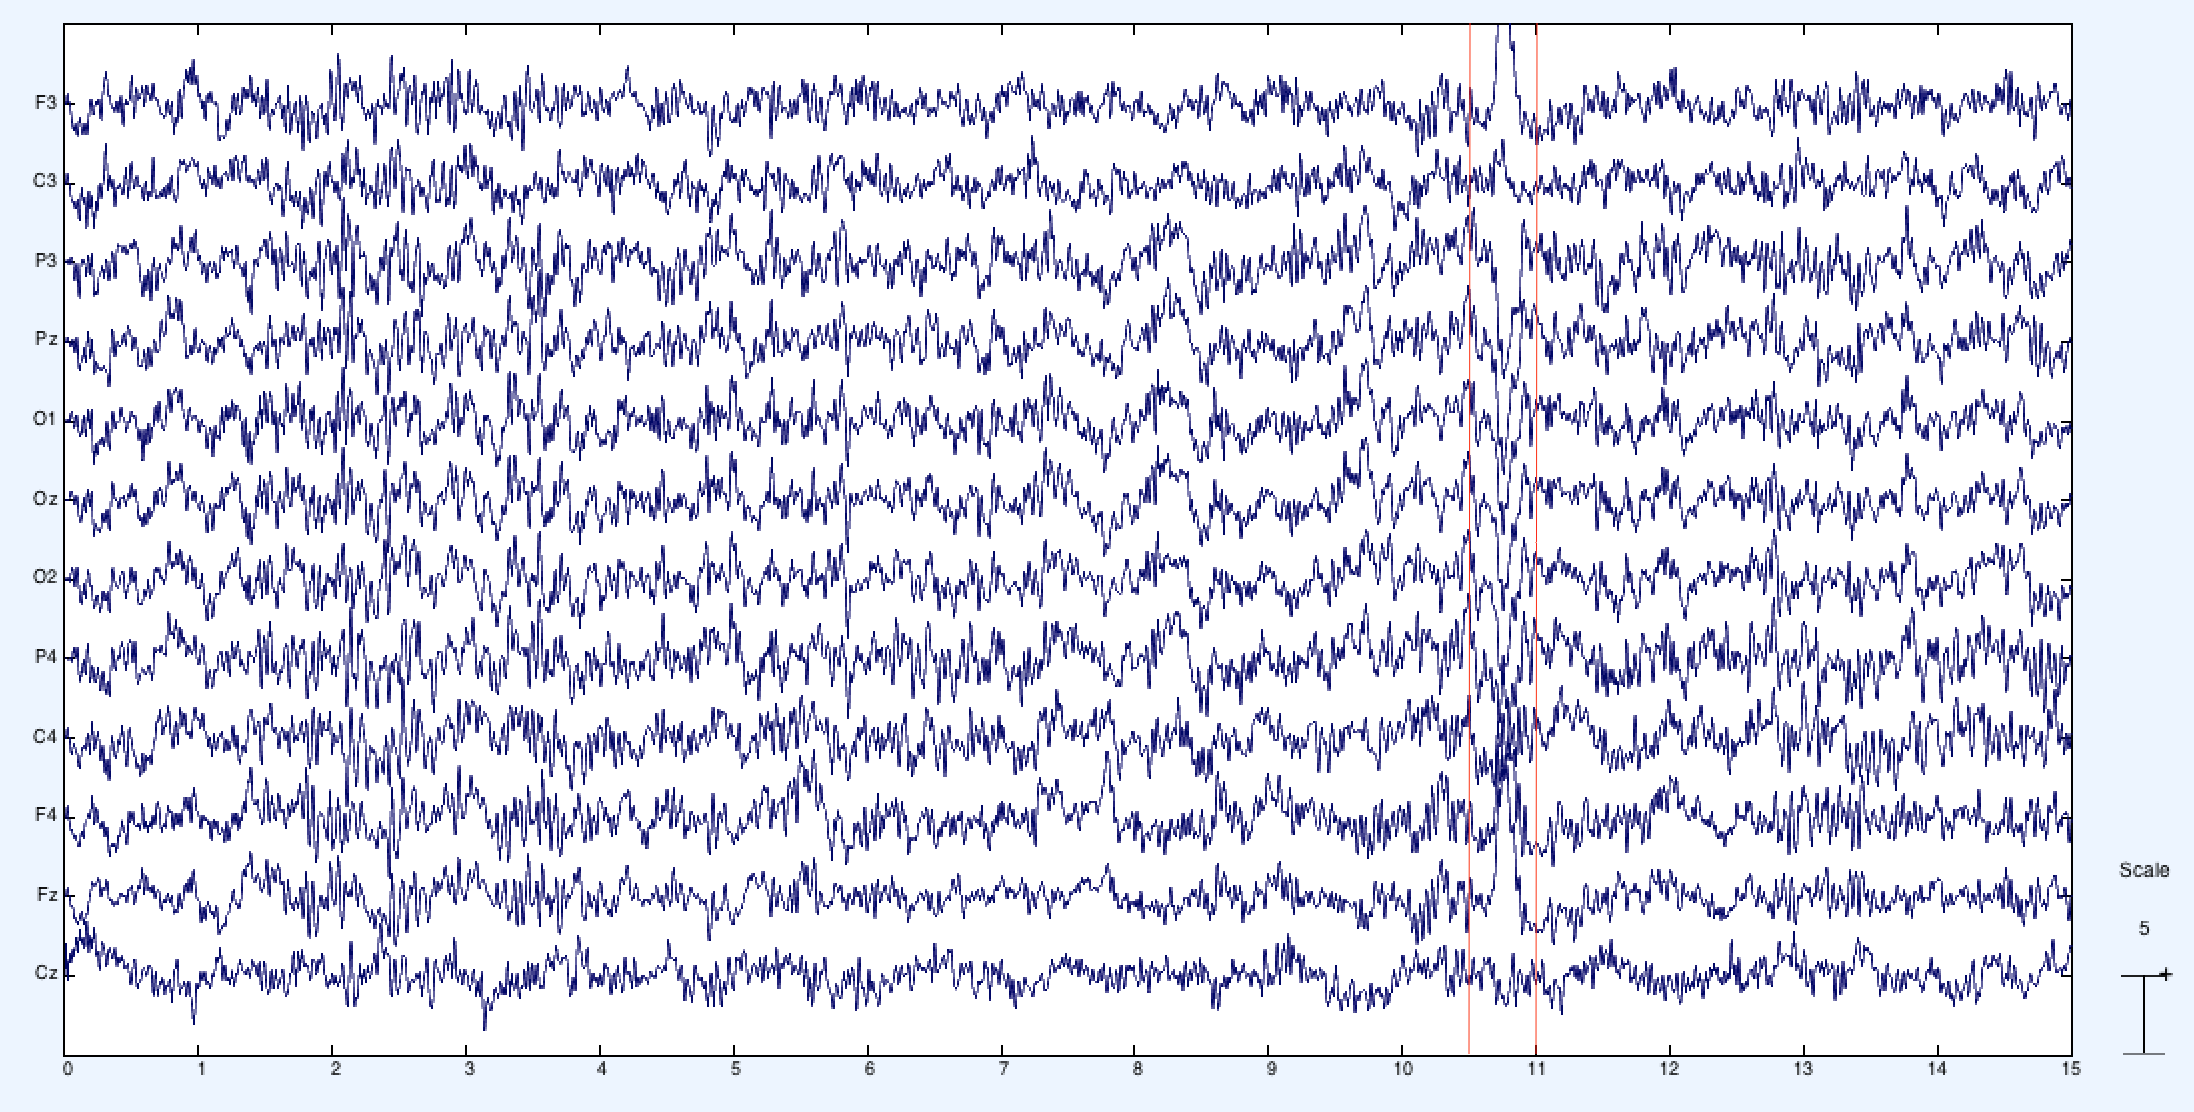
\includegraphics[width=\textwidth]{img/art.png}
			\end{center}
			\caption{Data stream with corrupted artifacts. The artifact region lies between the two red lines.}
		\end{figure}
				\begin{figure}[!h]
		\begin{center}
			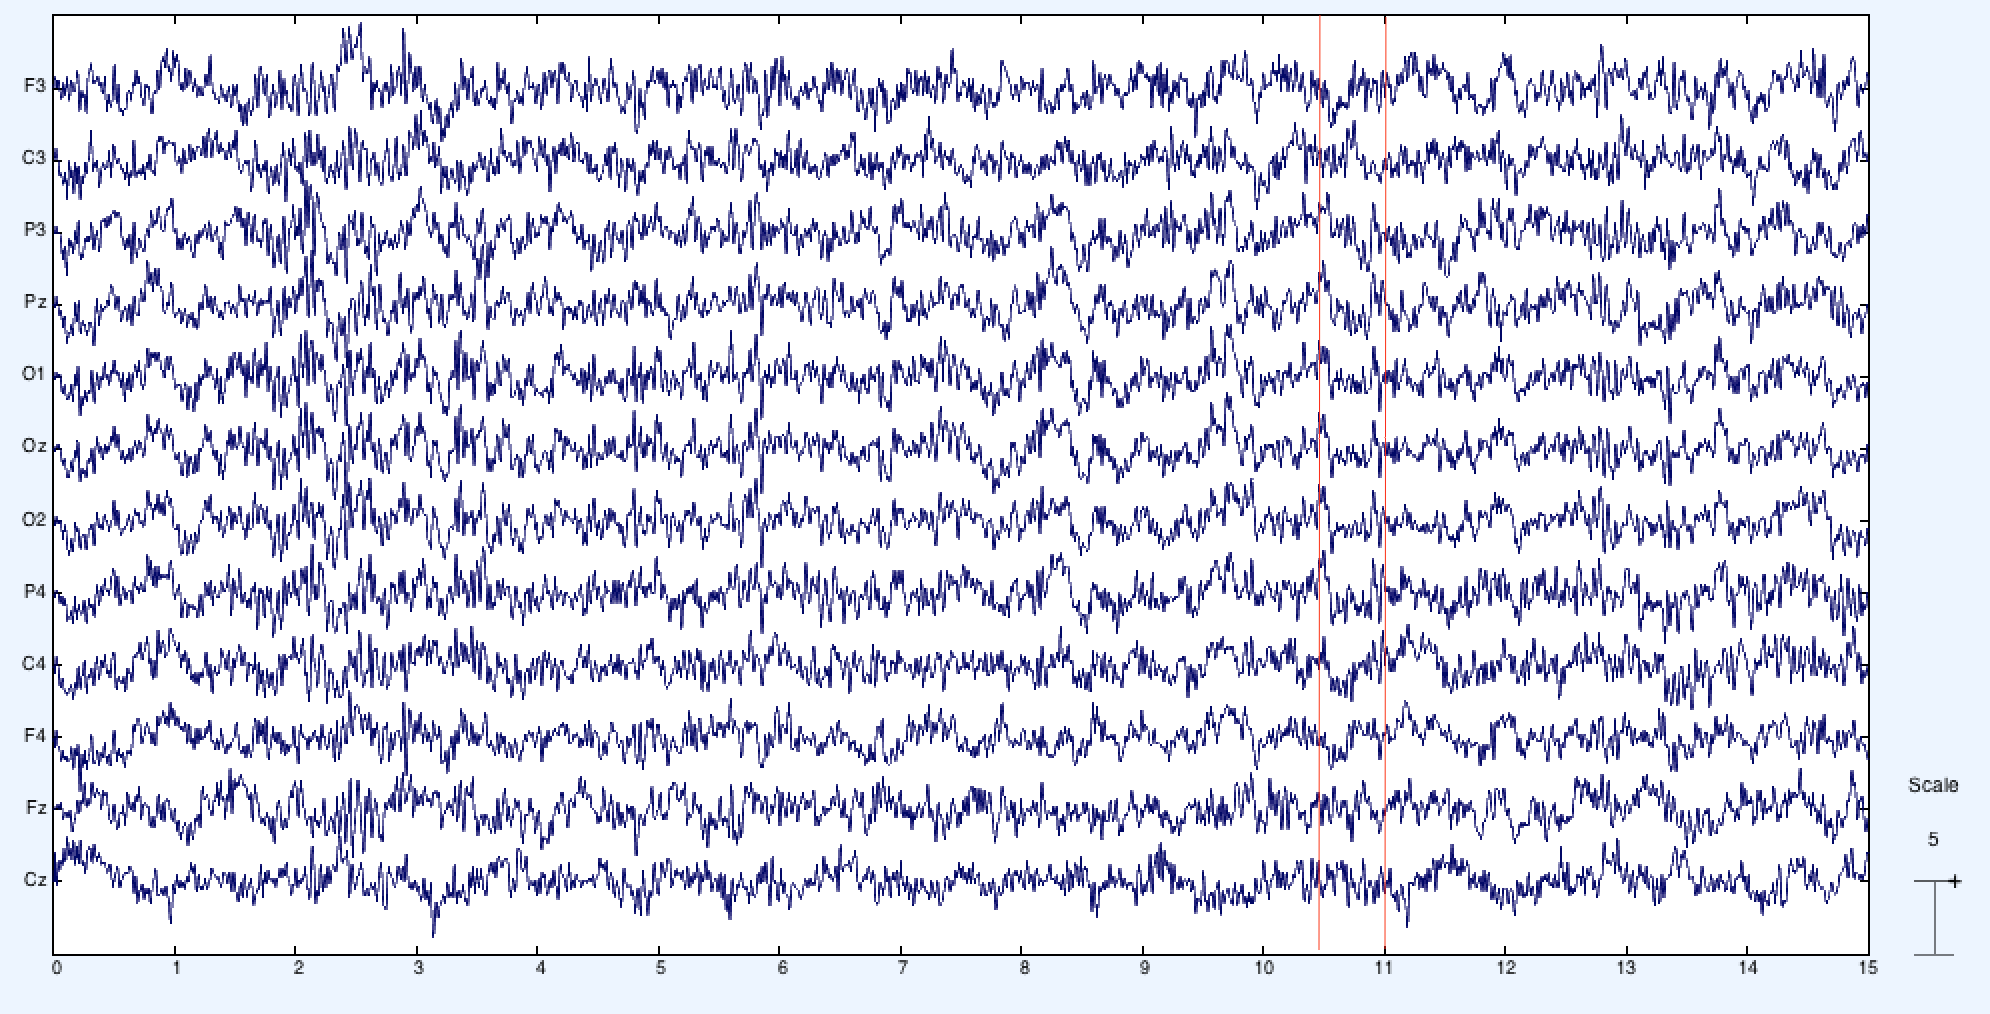
\includegraphics[width=\textwidth]{img/artrm.png}
		\end{center}
		\caption{Data stream with artifacts removed using ICA and MARA. The artifacts removed region lies between the two red lines.}
	\end{figure}
	Now we look into the effect of removing these two components. In Figure 8 and Figure 9, we can compare the differences to appreciate the power of MARA. Notably, at around 11 seconds in Figure 8 (the region within two red lines), there exists a clear indication of an artifact because we have some sharp amplitude changes which are more severe in the frontal lobe. We know this causation, because channels Fz F3 and F3 all show significant intensity changes. This effect should be attributed to eye movement as those channels are close to the eyes. After removing the eye movement component based on MARA, and we obtain the data in Figure 9, which has much more brain-like oscillations around 11 seconds.
	
	Furthermore, we normalize each input channel by 
	$$ \bar{u}_i(t) = \frac{u_i(t) - mean(u_i)}{max(u_i) - min(u_i)} i \in [1, 12] $$
	We understand this normalization approach for EEG data comparison across subjects is not optimal. This channel based method is adopted because EEG amplitude is also influenced by age, gender and race. It is hard to just normalize each channel within one single subject without jeopardizing target-related information. A more careful approach is to test the statistical difference of EEG amplitudes with respect to the three factors mentioned above and then do a parametric normalization if the differences are significant. However, it could also be that the amplitudes do not contain any information related to MLS, so we could remove the amplitude differences by matching the mean amplitudes of different subjects and conduct a normalization within each subject.
	
	Then, we remove the subjects whose EEG recordings are strongly influenced by artifacts and prior caffeine intake. Finally, we get rid of the relative MLS outliers which leaves us with 77 training samples.
		
	In the compression stage, we choose only 12 electrodes (F3 C3 P3 Pz O1 Oz O2 P4 C4 F4 Fz Cz), because  there are overlaps among electrode recordings. We use the 10-20 electrode placement system in our project, which uses numbers and letters to denote the brain regions \cite{klem1999ten}. The letters stand for the general areas: F(frontal), C(central), P(parietal) and O(occipital). The odd numbers mean represent the electrodes on the left hemisphere, and the even numbers represent the ones on the right. The exact locations of these electrodes on the scalp are shown in Figure 10. Then we will down sample the frequency of EEG recordings from 2048 Hz to 256 Hz. Recordings at extremely high frequencies do not have the relevant information about brain processes. We denote each electrode's recording by $c_i. i \in [1, 12]$. 
	All the preprocessing is done in Matlab using EEGLAB toolbox \cite{delorme2004eeglab}.
	
	\begin{figure}[!h]
		\begin{center}
			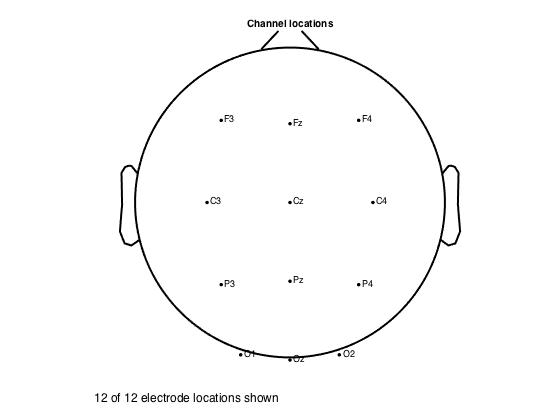
\includegraphics[width=0.7\textwidth]{img/chanLocation.jpg}
		\end{center}
		\caption{Locations of 12 selected electrode channels.}
	\end{figure}


\paragraph{Model Building} 

\begin{itemize}
	\item Encoding : After finished preprocessing the data, we define the relative MLS as $$ MLS = \frac{PreRMSE - PostRMSE}{PreRMSE}  $$
	The relative MLS is the main criterion that we use to label the subjects.   
	In Figure 11, we have the age (y axis) versus relative MLS (x axis) scatter plot.  For the relative MLS, the smaller the value is, the more one's motor skills can improve after training. We have three groups of subjects: yellow dots old high performing, blue dots old low performing and purple dots young high performing. All young subjects are considered high performing and among the old subjects, we use the median\footnote{The author understands that using median split is not the best encoding scheme here. One could use a range based method instead (more on this in section 7). For simplification, we go with the median split approach.  } to differentiate the high performing and low performing subjects. So after the encoding, the number of subjects in different groups is shown in Table 1, and the distribution of subject groups with respect to age and learning outcome is also depicted in Figure 11. The group labels are represented by their colors.
	
	\begin{table}[h]
		\centering
		\begin{tabular}{||c c ||} 
			\hline
			Group name & Subject count  \\ [0.5ex] 
			\hline\hline
			Young High (YH)  & 28 \\ 
			Old Low (OL) & 23  \\
			Old High (OH) & 24  \\ [0.5ex] 
			\hline
		\end{tabular}
		\caption{Subject counts in different group after encoding.}
	\end{table}
\nomenclature{\textbf{YH}}{Young High Performers} 
\nomenclature{\textbf{OL}}{Old Low Performers} 
\nomenclature{\textbf{OH}}{Old High Performers} 
	
	\item ESN construction:  We use 150 internal units as the starting point. We also use leaky neurons to update. Then we construct the teacher signal, a vector of size two by one, one element being one and the other being zero depending on which MLS group this subject belongs to. In the prediction phase, we first exploit the inputs $\mathbf{u}$ by using the updates rules defined in equation (2), and obtain $\hat{\mathbf{y}}$ of size 2 by T. The class of $\mathbf{u}$ thus becomes:
	$$ class_{idx} = max_{idx} [\sum_i^T\mathbf{y_{1i}}; \sum_i^T\mathbf{y_{2i}}] $$
	which is to sum the network outputs of each class label for a subject, and classify the subject as the class whose sum is greater.
	
	\item Training: We use the ridge regression with regularization which is discussed in section 2.1. In our experiment we train three binary classifier in total: young high performers vs old high performers, young high performers vs old low performers and old high performers vs old low performers.
	
\end{itemize}
\begin{figure}[h]
	\centering
	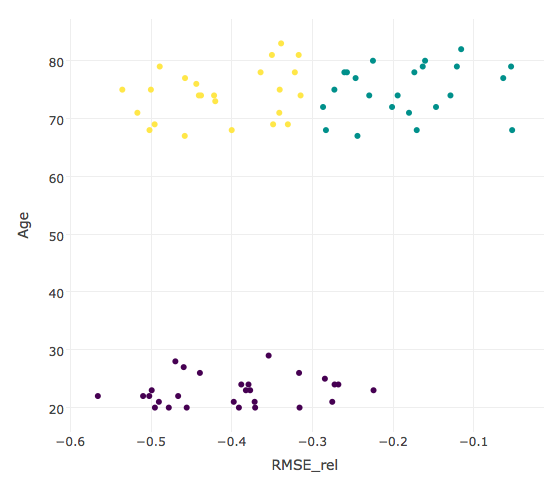
\includegraphics[width=0.6\textwidth]{img/scatter.png}
	\caption{The scatter plot of age vs the relative motor training improvement is shown. The y-axis is for age and the x-axis is for the relative motor training improvement. The smaller the x value is, the more one has improved after motor training. Yellow dots are OH; blue dots are OL; purple dots are YH.}
\end{figure}

\paragraph{Model Optimization}
As we know, EEG classification is prone to over-fitting, so after the model has been constructed, we fine tune the washout threshold, spectral radius, regularization and the leaking rate to get better results \cite{lukovsevivcius2012practical}. These four parameters are mostly dealt with, and the other parameters are disregarded in this experiment.


\paragraph{Stratified three-fold cross-validation}
In the evaluation phase, we use stratified three-fold cross-validation. Conventional cross-validation in our experiment setup would not work well because we only have two classes and a small number of samples in the order of tens, and therefore in the cross-validation phase mere random allocation of the data samples to different folds might lead to a situation where one class is only present in the testing but not in the training phase which will surely lead to bad performance. A good evaluation method should have both low bias and low variance and k-fold stratified cross-validation is in general better than the regular version \cite{kohavi1995study}. We only have 77 subjects and three groups, but we are constructing three mutual binary classifiers among these groups, which gives us around 50 subjects for each model. Hence we use the stratified three-fold cross-validation scheme to evaluate the model results. It turns out that the variations of errors between different folds and randomization differ a lot, and hence we always use the Mersenne Twister method with seed 0 \footnote{In Matlab, this can be set by `rng(`default')'.} to tackle this instability. 

\paragraph{Parameter selection}
The washout threshold stays reasonably stable while other parameters are changing, so we pick the washout threshold first. The deciding factor is when we move back the threshold, the classification result does not fluctuate too much, and at the same time that the internal neuron responses remain relatively stable. The first value of such a point should be the washout threshold. In our experiment, we found out 550 to be a good enough threshold.

The parameter values for the YH vs OL performers and YH vs OH are quite similar so we just showcase the validation error behavior on the YH vs OL model. 

After having set the washout threshold, we first do a parameters manual search to locate the range of the values for the later systematic tunning, then we do a grid search on the leaky rate $\alpha$ and the spectral radius $\rho$. The final step is to increase the number of internal units to improve accuracy. In this project, the number of units actually has a strong influence on the performance due to the complexity of brain data.

Even with a network of size 1000, we are still not overfitting yet as one can see from Figure 12. On the x-axis, we have regularization term starting from 0.0000001 to 0.01. For each iteration we multiply the regularization term by 5. Neither the training nor testing error benefits from more regularization. We also found out that the bias term scale does not make a difference here, so we will just use one.
\begin{figure}[h!]
	\centering
	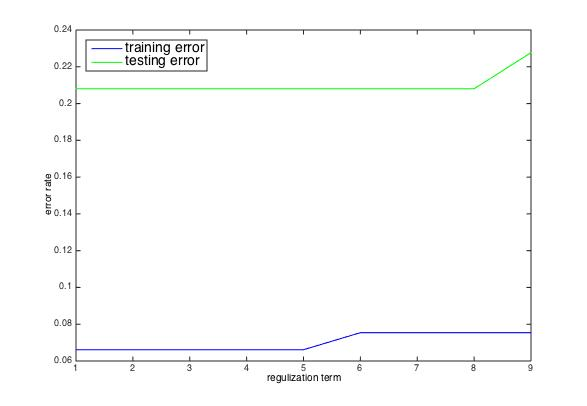
\includegraphics[width=0.7\textwidth]{img/reg.jpg}
	\caption{Training and testing error with respect to regularization term. The regularization term starts from 0.0000001 to 0.01 (0.0000001 being 1 and 0.01 being 9). Each value to the right on the x-axis, the regularization will be multiplied by a factor of 5.}
\end{figure}

\section{Results}
\subsection{Network dynamics}
In Figure 13, we have two sample network outputs for both the right and wrong classifications. The simulated class signals are the network outputs and the true class signals are the ground truths. Clearly, for the correctly classified output on the left, the range for the network output spans wider between 0 and 1, however for the wrongly classified output, the range for the network output is more narrow and the two simulated class signals swap the leading position more frequently.

\begin{figure}[h!]
	\centering
	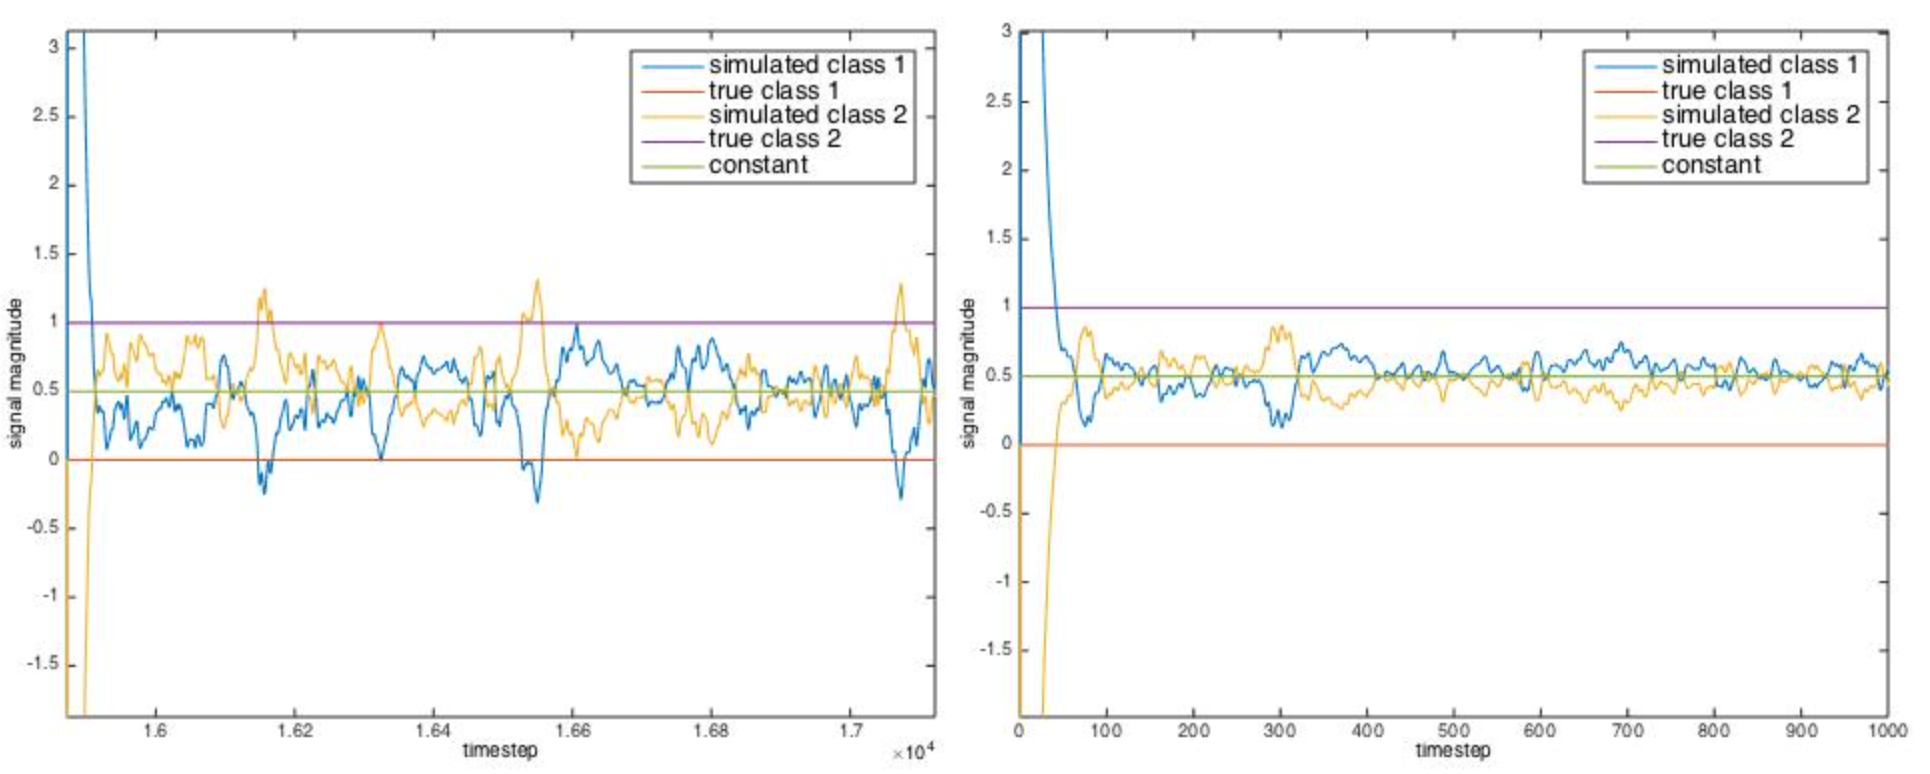
\includegraphics[width=1.05\textwidth]{img/simulation.png}
	\caption{The left chart is a sample network output that has been correctly classified, and the right chart is a sample network output that has been wrongly classified}
\end{figure}

We then take a look at the interval units dynamics. In Figure 14, we can observe that all inputs vary between -0.5 and 0.5, and it is hard to find a correlation between the inputs and interval units just by eyesight. As for the internal units dynamics in Figure 15, different units have different ranges and show different frequencies as well, for instance, unit 42 seems to change faster than unit 34. The amplitudes of the internals units are still narrow, not making use of the full range between -1 and 1 either.
\begin{figure}[h!]
	\centering
	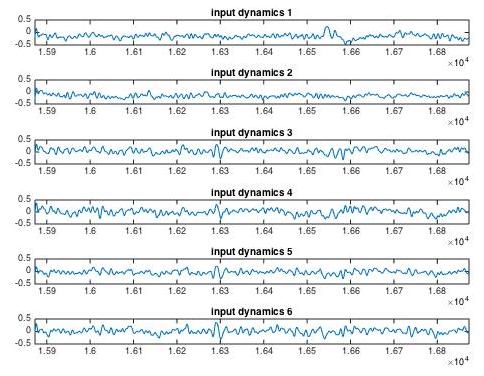
\includegraphics[width=0.85\textwidth]{img/rightIns2.jpg}
	\caption{Sample input dynamics for a correctly classified example.}
\end{figure}
\begin{figure}[h!]
	\centering
	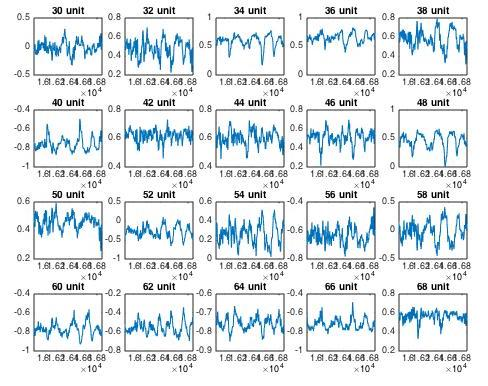
\includegraphics[width=0.85\textwidth]{img/rightIns.jpg}
	\caption{Sample network dynamics for a correctly classified example.}
\end{figure}

\subsection{Model performance}

The parameters used are $\rho = 0.4 \text{ and } \alpha = 0.1 $ for OH vs YH on a network whose internal units are of size 1500, and the parameters for the OL vs YH model are quite similar just changing $\rho$ to 0.1. However, for the OH vs OL, the author could not find good enough parameters to make the testing error better than random chance. Regularization is set to zero for all models. 
\begin{table}[h!]
	\centering
	\begin{tabular}{||c c c||} 
		\hline
		Model type & Training Error & Testing Error \\ [0.5ex] 
		\hline\hline
		model a: OH vs YH & 0.0947 & 0.2070 \\ 
		model b: OL vs YH & 0.0659 & 0.2092  \\
		model c: OH vs OL & 0.1667 & random chance  \\ [0.5ex] 
		\hline
	\end{tabular}
\caption{Training and testing errors for different models.}
\end{table}

From Table 2, one can see model a and model b achieve similar performances, albeit model c is hopeless. 

A confusion matrix is constructed by summing up the target and output labels across our stratified three-fold classification. Let us look at the matrix for model a first (Figure 16 left). There exists a systematic preference towards YH as $37.5\%$ of OH are misclassified as YH. The accuracy for OH ($88.2\%$) and the recall for YH ($93.1\%$) are reasonably good, however the accuracy for YH ($75.0\%$ ) and recall for OH ($62.5\%$) are worse off.
The confusion matrix for model b (Figure 16 right) follows a similar pattern, there exists a systematic bias from OL to YH, given that not a single YH has been misclassified as OL but about $20.8\%$ of OL are misclassified as YH. Both accuracy for OL and the recall for YH are perfect but the accuracy for YH ($72.5\%$) and recall( $54.2\%$) for OL are less satisfying. As for model c, no strong bias is observed in the misclassified samples.
\begin{figure}[h!]
	\centering
	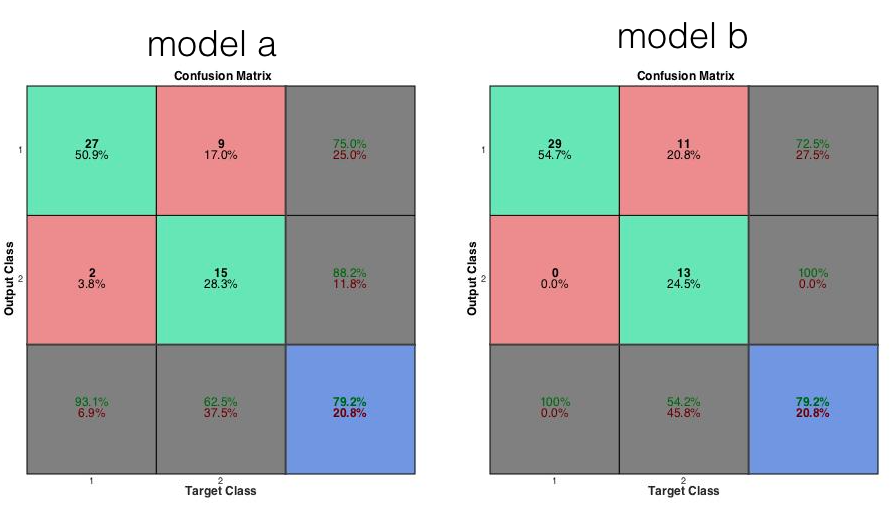
\includegraphics[width=\textwidth]{img/confusion.png}
	\caption{Confusion Matrix for model a and b. For model a, class 1 is YH, and class 2 is OH. For model b, class 1 is YH, and class 2 is OL. The green texts are marginal correctness percentages and the red ones are the error rates. The top left 2 by 2 matrix shows the raw count and classification results and their corresponding percentages within the overall population. The gray column on the right shows the accuracy of each predicated class, while the row at the bottom shows the accuracy of each true class. The cell in the bottom right shows the overall accuracy. }
\end{figure}


Interestingly, If we use model b to test on the OH group, model b will predict that all subjects in OH belong to YH. If we use model a to test on OL group, model a will categorize all subjects in OL into OH.


\section{Discussion}
\paragraph{Engineering analysis}
As usual, we first talk about the engineering side and then go on to the neurological side.  Model a and b, which classify between young and old subjects, perform reasonably well, meaning, being able to separate between the YH vs OL and YH vs LH, which human experts are not able to do. So ESNs can indeed pick up some spatiotemporal features that EEG contains.
 
 Now let us look at pitfalls and possible extensions. As we have seen, regularization term does not help with the performance much when the network has 1000 internal units based on Figure 12, in which neither the training nor the testing error improves with respect to the regularization coefficient. This could imply that the network is still underfitting. This is not too surprising, when one considers the amount of data we have. Each time series has 15k timesteps after down-sampling, and we have 12 channels for each series. For each model, there are approximately 50 subjects to work with, and we are using three-fold cross-validation which means around 30 subjects are used for training, which leads to 15k * 12 * 30 = 5.4M number of data points for training.

When we look at the network output in Figure 13, the network decision is quite uncertain when dealing with complex data like EEG. Although for the rightly classified data, we can see the amplitude of the output is greater, and leading position of the two competing class signals switches less frequently in comparison to the one that is wrongly classified.  

From both Figure 14 and Figure 15, we notice the effects of inputs not being ``well normalized'' in a sense that the inputs are not making use of the full range between -1 and 1. We already discussed this issue in section 2.2 and possible extensions by using parametric normalization in order not to lose target-related information. As a consequence of the current implementation, the network will surely find it easier to classify the ones with strong amplitudes, hence for the ones that have small amplitudes, the internal units are not making use of the full range between -1 and 1 either. Therefore, a more complicated normalization routine is needed to hopefully ameliorate the classification performance.

Finally, we have come to discuss the bias encountered in the confusion matrix in model a and b. Particularly in model b, all the misclassified subjects actually belong to OL, and YH can be perfectly separated. One possible explanation might be the uneven distribution of training data, given we have 28 YHs and only 23 OLs. 


\paragraph{Neuroscience analysis}
Based on the classification results, we can say that something is different between the young and old groups that enables model a and model b to perform well. The difference between OH and OL is hard to tell, since model c cannot perform better than random chance. 

Another observation is, if we use model b to do a test on OH, the network will classify all the subjects to YH, which is to say that the network thinks the brain activity of the OH subjects are more similar to the ones of YH as compared to OL. On the other hand, model a (trained on YH and OH) classifies all OL to be OH, which indicates that indeed OH are similar to YH. Although our model c (trained between OH and OL) fails, based on the above facts, we are still able to discriminate OH and OL by using model b alone. The decision procedure can be as simple as: 

\begin{lstlisting}[language = Matlab, caption = Classification function between OH and OL]
subject1 = loadSubject();
if (modelB.predict(subject1) == YH)
	subject1.class = OH;
else 
	subject1.class = OL;
end
\end{lstlisting}

In summary, we know the high performers' brains in young and old subjects work differently in order to enable model a to reach high accuracy. Also among the old subjects, high and lower performers' brains also work differently in order to enable listing 1 to discriminate between OH and OL.

\section{Conclusion and future work}
Previously ESNs have been shown to be useful for epileptic seizure detection. This project is yet another successful application of using ESNs on EEG data. We also observe evidence that proves the existence of different neurological groups for MLS.

Furthermore, this guided research is also an attempt for correlation analysis in the realm of end-to-end ML techniques. ML techniques are powerful, and they will become even more so, if we understand what is going on behind the scene, in addition to merely focusing on the model performance without much understanding. 

Possible future works include constructing the gradient target value for MLS instead of using binary classification to have more conclusive results. Also importantly, one can apply the notch filter and proper normalization scheme to see how much more accurate the classifiers can get. This extension should in theory help to develop a working classifier between OL and OH, since we already have an indirect routine to differentiate these two groups as shown in Listing 1. 

\begin{figure}[h!]
	\centering
	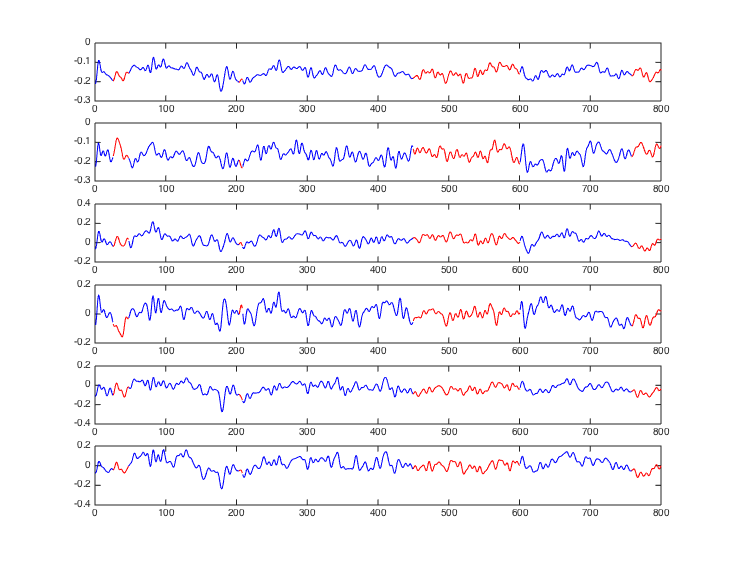
\includegraphics[width=0.8\textwidth]{img/futureVisu.png}
	\caption{A mini example for classified input signals in model b. Red means class 1 and blue means class 2.  }
\end{figure}
One could also further develop general statistical frameworks of how to construct different classifiers and by analyzing their decision boundaries for hypothesis testing and explore their mathematical nature. Perhaps something more feasible that can be done is to develop ML-assisted techniques for scientific discovery. We have shown that there are differences among OH, OL, and YH, but the exact difference is unknown. One nice thing about ESNs is that we can visualize and internal dynamics a lot easier than ML methods which often have parameters of on the order of millions. We can visualize input channels, reservoir dynamics with the help of decision vector as shown in Figure 17. The colors are given based on the outputs of the network, then the human experts can directly observe what kind of activities that the networks consider as class one or class two to help with their investigation. We will probably obtain more insights by averaging the EEG data, to find out the most common pattern being classified to a particular class, if we are determined to find out the analytical explanations. In this ML-assisted fashion, the myths of black-box modeling should start to unfold.




%: References

\clearpage
\newpage



\bibliographystyle{unsrt}
\bibliography{eeg_report}



\end{document}



